    \chapter{B-Spline Theory} \label{appbsp}

        From mathematical point of view , a curve which is generated by using
        the vertices of a defining polygon is dependent on some interpolation
        or approximation scheme to establish the relationship between the
        curve and the polygon.~\cite{Roger}.This scheme is provided by the
        choice of a basis or weighting function.

        Bspline is a series of polynomial splines joined end to end.
        ~\cite{PHIGS}
        Each of these splines is called a span of the curve.One of the important
        advantages of the Bspline curves is that you can define these piecewise
        polynomials as a single curve, and control the continuity at the joints
        between them.
        Bspline equation in terms of parameter t can be written as

            $ C(t) = \sum_{i=1}^{n}B_{i,k}(t)P_{i} $

        where,\begin{itemize}
            \item
            $n$         =   number of control points.
            \item
            $P_{i}$     =   control points.
            \item
            $B_{i,k}$   =   Bspline basis functions.
            \item
            $k$         =   order of the curve.
            \end{itemize}
            Order indicates the number of adjacent control points that influence
            the position of any point on the curve.In second order curves only
            two control points determine the location of the points along the
            curve segment.In the third order curves , three adjacent control
            points determine the location of the control points of the curve,
            and so on for higher orders.(see Figure ~\ref{bsporder}

        \begin{figure}[htbp]
%            \centerline{\psfig{figure=bspord.ps,width=4.0in,height=4.0in}}
	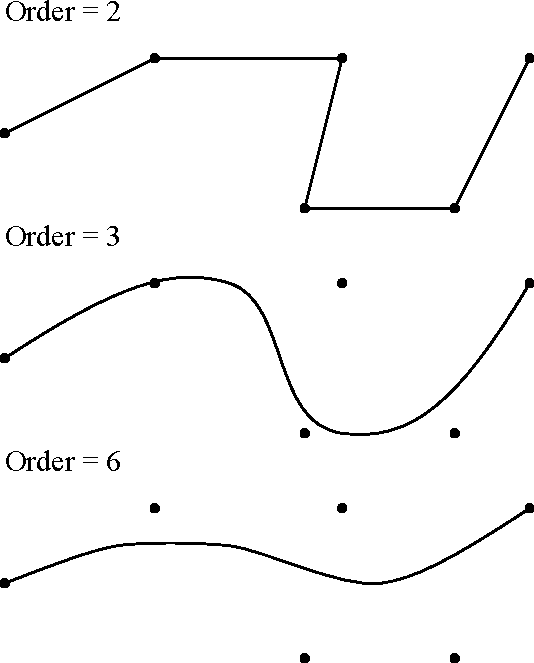
\includegraphics{BSPORD.pdf}
            \caption{B-slpine curves with different orders}
            \label{bsporder}
        \end{figure}


            Bspline surfaces are defined by the same Bspline basis function
            as Bspline curves.In curves, parameterization is done with one
            variable while in surfaces it it done with two.

            $ S(u.v)  = \sum_{i=1}^{n}\sum_{j=1}^{m}B_{i,k}(u)B_{j,l}(v)P_{i,j}$

            To completely define the surface we need

                \begin{enumerate}
                \item
                Order of the curves in both u and v direction
                \item
                Control net
                \item
                Knot vectors for both u and v dimensions
                \end{enumerate}




